% Euclidean Handout Number One Fall 2013
\documentclass{tufte-handout}

%\geometry{showframe}% for debugging purposes -- displays the margins

%%%% Packages to make things pretty
\usepackage{amsmath,amsthm}
\usepackage{booktabs}
\usepackage{graphicx}
\setkeys{Gin}{width=\linewidth,totalheight=\textheight,keepaspectratio}
\graphicspath{{graphics/}}
\usepackage{units}
\usepackage{fancyvrb}
\fvset{fontsize=\normalsize}
\usepackage{multicol}
\usepackage{pdfpages}

%%%% Theorem Evironments
\theoremstyle{definition}
\swapnumbers
\newtheorem{problem}{Problem}[section]
\newtheorem{conjecture}[problem]{Conjecture}
\newtheorem*{definition}{Definition}
\newtheorem*{theorem}{Theorem}
\newtheorem{question}[problem]{Question}
\newtheorem{challenge}[problem]{Challenge}
\newtheorem*{postulate}{Postulate}

%%%%%

\title{Euclidean Geometry:\\An Introduction to Mathematical Work}
\author[Math 3600]{Math 3600, Fall 2013}
\date{August 2013} 

\begin{document}

\maketitle

\begin{marginfigure}
    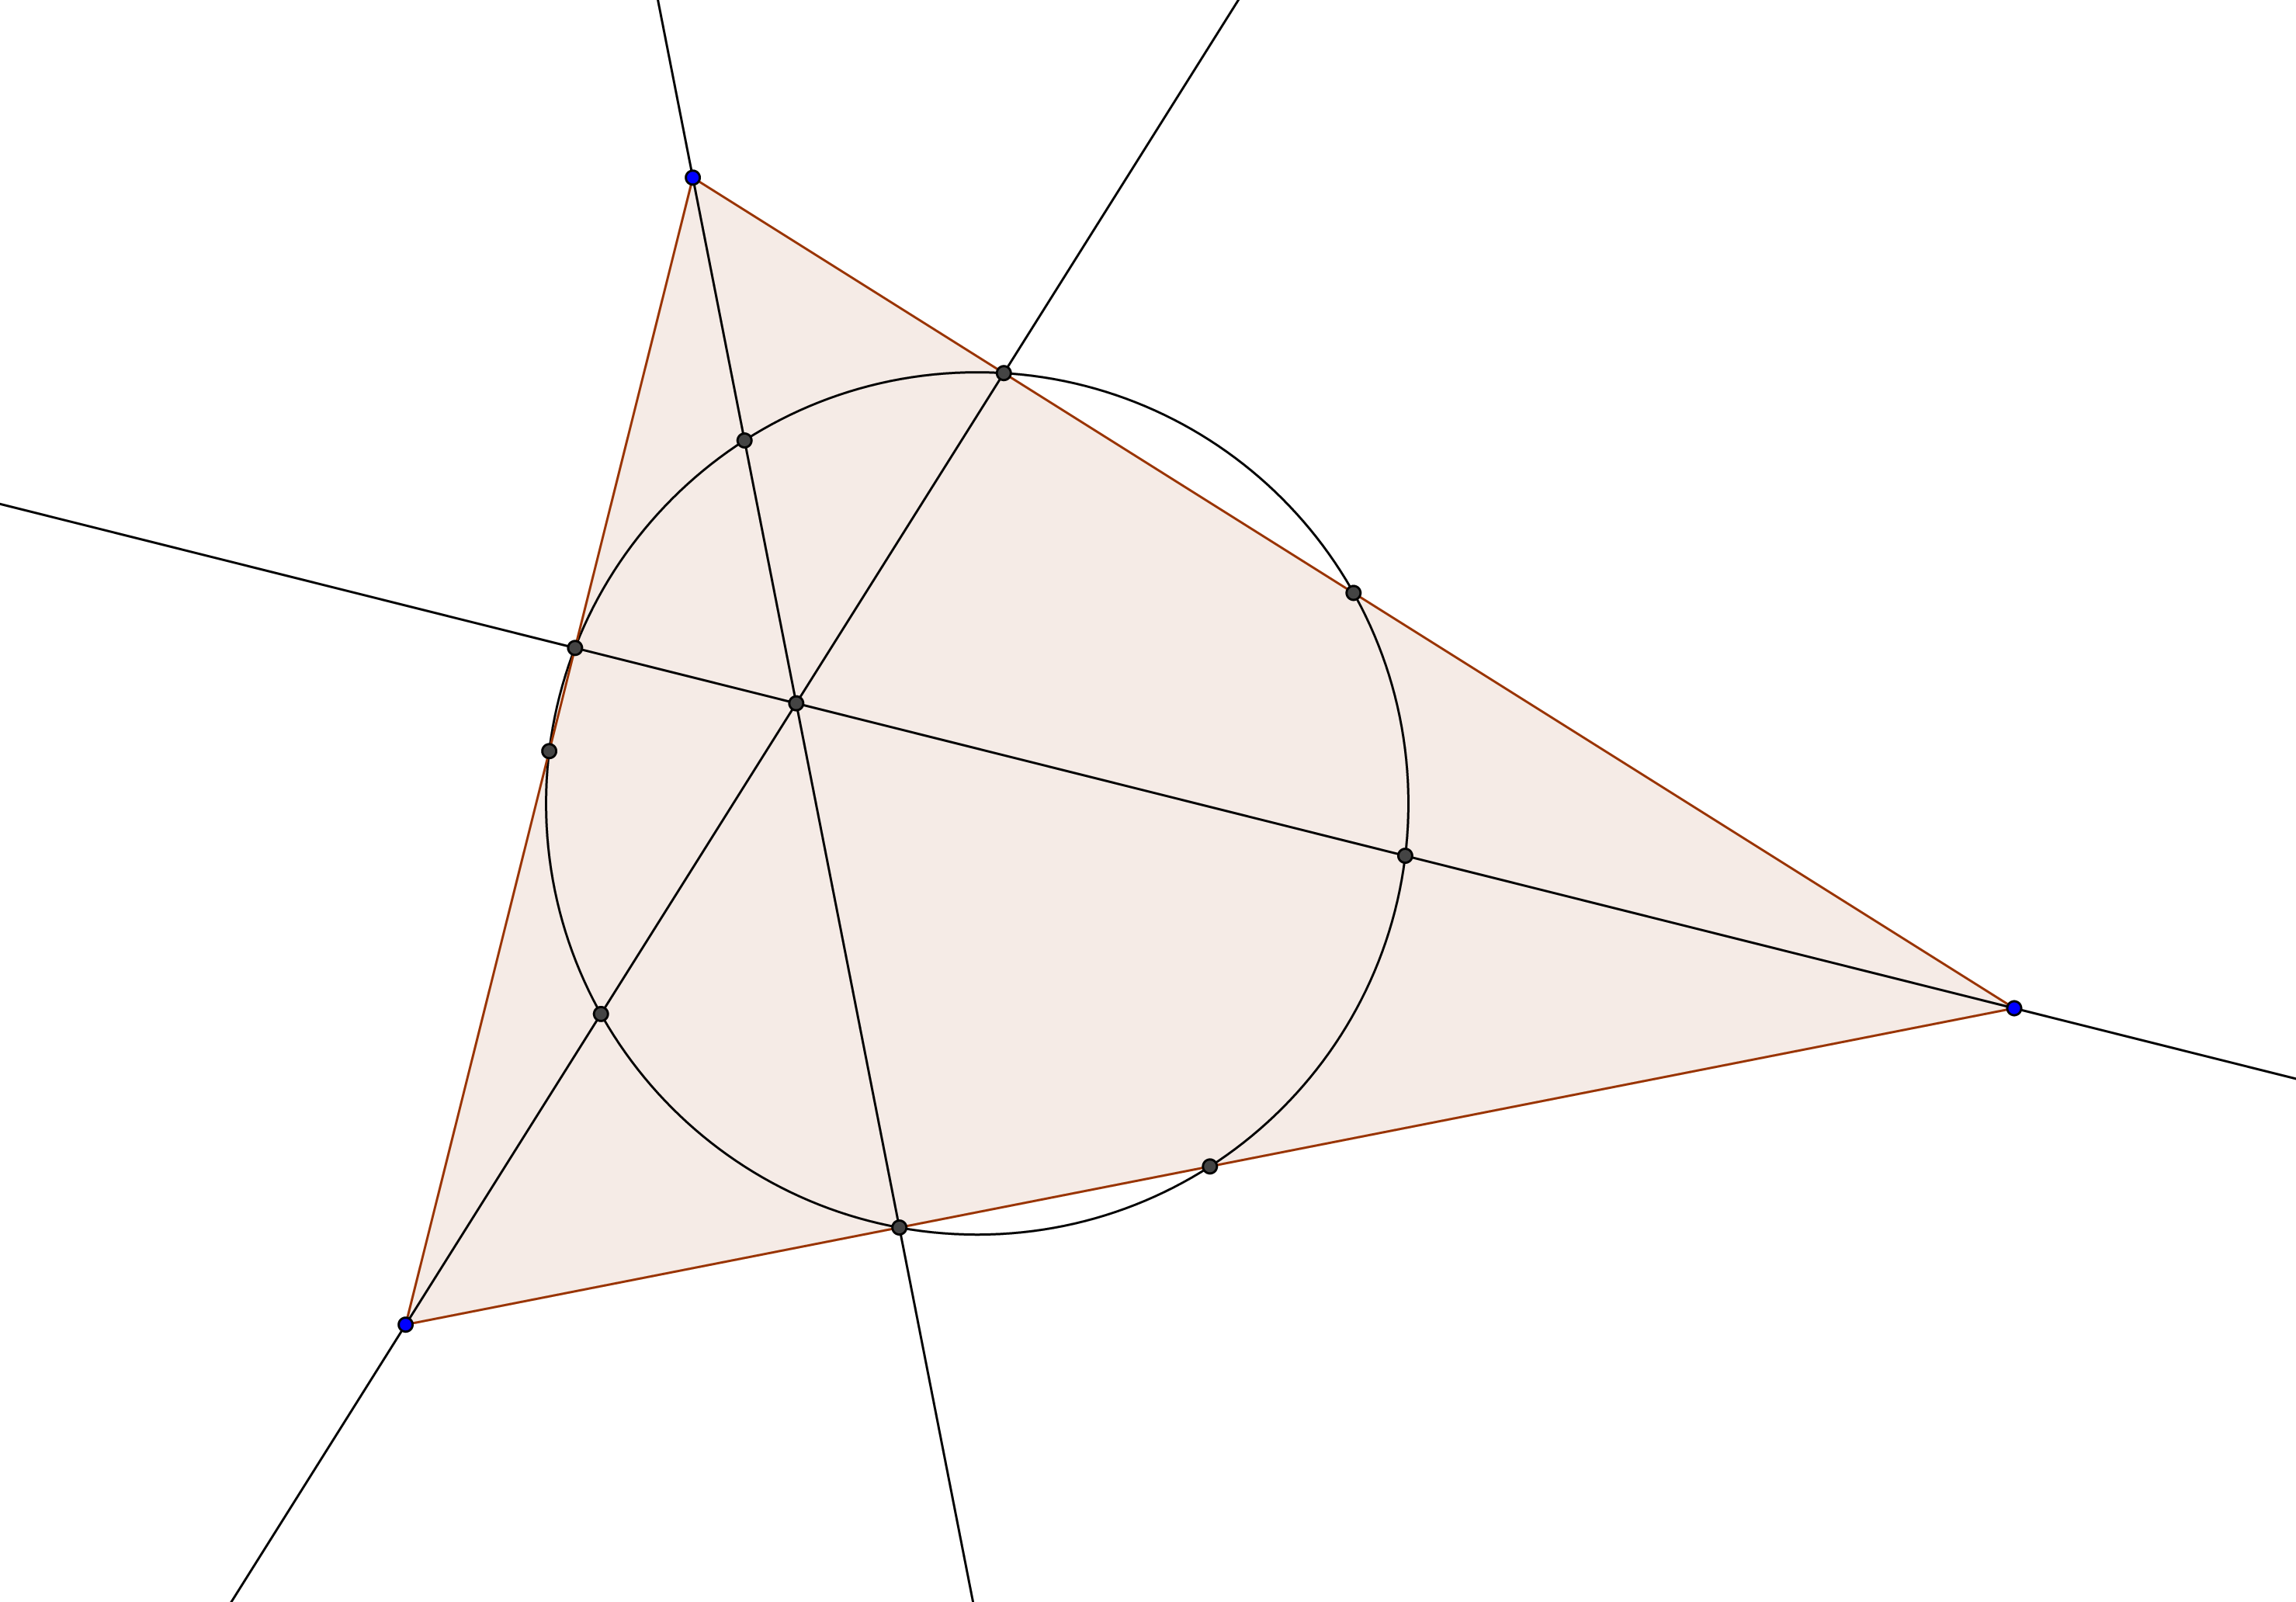
\includegraphics{NPC}
\end{marginfigure}


%%%% \setcounter{section}{-1}
\section*{Introduction}

We have two goals this semester: 
First and foremost, we shall learn to do mathematics independently. 
Also, we shall study planar Euclidean geometry. 
Euclidean geometry has been used throughout recorded history as a way to learn to do mathematics and as a way to sharpen thinking skills like problem solving and making logical arguments. 
We shall join the tradition.
\marginnote{ Euclid's \emph{Elements} is the world's oldest surviving textbook, and still one of the best, so we shall study it.}

\subsection*{About the Mathematics}
The general plan of mathematical work has a recurring structure. 
It starts when somehow, some way, a person has had an idea about a bit of mathematics and has asked a \emph{Question}. 
Perhaps, this person even believes that he or she knows the correct answer and is brave enough to share it publicly, and then we have a \emph{Conjecture}.
Now we have a job to do in two parts. 
First, we must decide what we believe the answer is. 
This is a lot of hard work where you look at examples, draw pictures, use your imagination and any other tools at your disposal to make up your mind. 
Second, you must find an argument supporting your answer. 
This argument is called a \emph{proof}. 
We will spend almost all of our time on proofs this term. We will think them up, share them with others and argue over their correctness. 
When we as a community agree that a proof is correct, then the statement we started with will be called a \emph{Theorem}.
To restart the cycle, we collect observations and ask new questions based on what we have just accomplished.
\marginnote{\dots Or \emph{failed} to accomplish.}

\newthought{The \emph{Elements}} is full of theorems and proofs. 
\marginnote{In fact, it has little else in it.}
 You can use these as examples and guides for how a proof should look, but keep in mind that Euclid lived a long time ago. 
 What we have now is translated from ancient Greek to English, and the translator did his job about a century ago, so the language is a bit odd. 
I want you to write your proofs in standard English prose. 
So, look at Euclid's first theorem and its proof as given by Heath's translation of Euclid's original, and compare it to this update that I'll write to show how one might do it today. 
Note that the descriptions given are pretty clear and match the figure.
Generally, one should write as if there is no diagram, and then draw one for the reader anyway.

\begin{quotation}
\begin{theorem}[Proposition One] 
If $AB$ is a line segment, then there exists an equilateral triangle $ABC$ having $AB$ as one of its sides.
\end{theorem}

\begin{proof} 
What we really need is a very special point $C$. 
The idea is to find the required point as the intersection of two circles.

By Postulate 3, there exists a circle $\odot AB$ with center $A$ which passes through $B$, and also a circle $\odot BA$ with center $B$ which passes through $A$. 
These two circles intersect twice.
Choose one of the points of intersection and call it $C$.
By Postulate 1 we may draw the segments $AC$ and $BC$.
This forms a triangle $ABC$, by definition of a triangle.
\begin{marginfigure}
    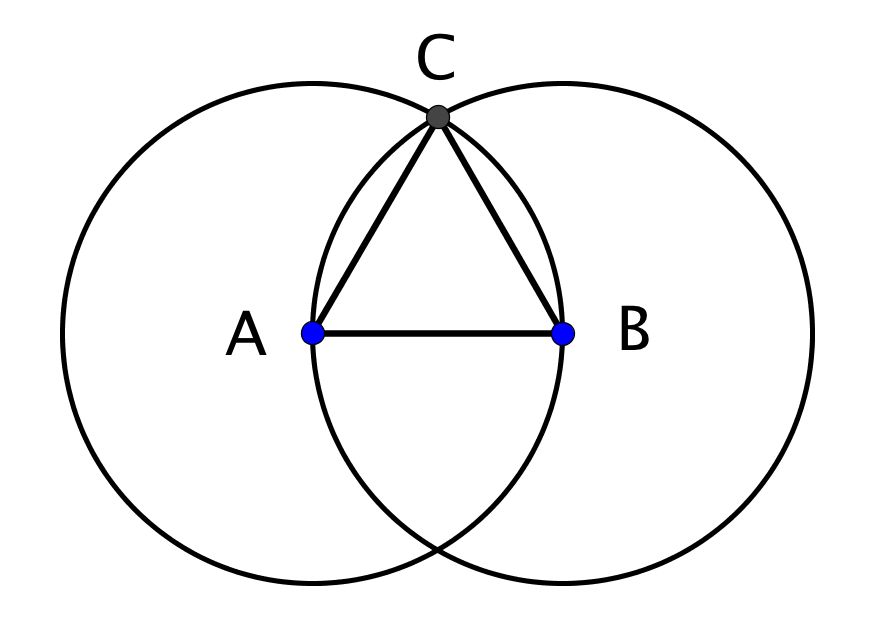
\includegraphics{Euclid1_1}
    \caption{Euclid's First Figure}
\end{marginfigure}
What remains is to show that the three sides of the triangle are mutually congruent.

Since $C$ and $B$ both lie on circle $\odot AB$, by the definition of a circle, segments $AC$ and $AB$ are congruent.
Similarly, since $C$ and $A$ both lie on circle $\odot BA$, by the definition of a circle, segments $BC$ and $AB$ are congruent. 
Now, by Common Notion 1, since $AC$ is congruent to $AB$ and $AB$ is congruent to $BC$, we see that $AC$ is congruent to $BC$. 
This means that all three of the sides of triangle $ABC$ are mutually congruent, so $ABC$ is equilateral, by definition. 
This concludes the proof.
\end{proof}
\end{quotation}

\newthought{Note that Euclid} phrases his result as a construction problem and the ``proof'' has two parts: the first is a routine for doing the construction and the second is an argument for why it works. 
The more modern view is to see this as an \emph{existence} result with a \emph{constructive proof}.



\newthought{Also, note how} the proof works. 
Each statement is justified by reference to something we have already agreed upon. 
Since this is our first result, we can only refer to assumptions that we have agreed upon in advance. 
These assumptions are called \emph{Postulates} or \emph{Axioms} or \emph{Common Notions}. 
Also, we have \emph{definitions}, which are shorthands telling us that when we use a certain word, it has exactly some specific meaning.
\marginnote{We will spend a lot of time thinking about the way mathematical definitions work.}
Later proofs can (and will) also rely on previously proved theorems to justify some of their steps.

This way of working is called the \emph{Axiomatic Method} and is characteristic of mathematics.
``Axiomatic Proof'' is what distinguishes mathematics from practically everything else.
It can feel a bit unnatural at first, but you will get used to it.

\newthought{Finally, notice that} one step really isn't justified.
Did you see it when reading? 
It is easier to spot in my writing than in Euclid's version. 
If you didn't notice it, go back and try to find it before reading further. \\

\vfill
\pagebreak

\newthought{What is the gap} in the proof? 
Euclid just assumes that the two circles $\odot AB$ and $\odot BA$ intersect twice. 
This seems obvious from the picture he draws, but nowhere in his list of Postulates and Common Notions does he say anything about how two circles should intersect! 
What is needed here is another assumption, which I hope you will be willing to believe, called the ``circle-circle intersection property.'' 
\begin{postulate}[Circle-Circle Intersection Property] 
If circle $C$ contains a point in the interior of a circle $D$ and also contains a point in the exterior of circle $D$, then circle $C$ and circle $D$ meet at two points. 
\end{postulate}

There are lots of little things like this in Euclid's work.
It is hard to know how picky one wants to be. 
My feeling is that we should just note what our assumptions are as we go, and to try to keep the list of assumptions relatively short and simple. 
But mathematicians are habitually picky, and you should get in the habit of reading with a very critical eye.

%%%%%%%%%%%%%%%%%%%%%%%%%%%%%%%%%%%%%%

\section*{Advice About Doing Mathematics}
 It is impossible to summarize all one needs to know to do mathematics successfully, and I don't even pretend to know how to write an exhaustive list.
 \marginnote{I am sure that I have much to learn, still.}
 But I want to give you some basic advice anyway. 

\subsection*{Getting Stuck}
If you are really working at a level that will help you improve, you will get stuck and confused a lot.
Being confused is the first step to learning.
\marginnote{Suckin' at something is just the first step to being sorta good at something.\\
---Jake the Dog, \emph{Adventure Time}}
When you feel stuck, come talk to me.
I like teaching, I like geometry, and I want to help you get through this.
I am sure that I can nudge you in a productive direction when you get stuck.

\subsection*{Good Work Habits} 
Work every day, at the same time each day if you can.
Mathematics doesn't happen fast, so you must give yourself time to get to your goal.
Also, when you have an idea, take notes.
Most ideas don't work, but some that don't work now might work for another problem later.
It is a terrible waste of time to `reinvent the wheel' for each problem.
Keep a geometry research notebook.

\subsection*{Collaboration}
Most mathematicians and students of mathematics find great value in talking to others about mathematics.
I encourage you to do this, too.
Getting the most out of a collaboration requires two things:
\begin{itemize}
\item Work hard on your own first. 
\marginnote{No one wants a dead weight collaborator.}
You can't have a conversation if you don't know what is going on and have no ideas to share. 

\item Give credit where it is due. 
If you talked to someone about a problem and then you solved it, you should mention that conversation when you give presentations of your work (orally or in writing).
\marginnote{Selfish people shed collaborators, while generous ones keep them.}
If you worked together through the whole process, then you should consider \emph{joint authorship} on any written work.

\end{itemize}


\subsection*{Expectations} 
The expectations for this class are simple.
You should come to class every day prepared to discuss the mathematics. First and foremost, this means:
\begin{quotation}
\textbf{\emph{You should try to solve every problem}}.
\marginnote{TRY TO SOLVE EVERY PROBLEM.}
\end{quotation}
You must solve several problems by the end of the semester.
When you solve a problem, write up your arguments before class so that you are ready to present.
During class when someone else is presenting, pay attention.
Try to catch  mistakes, both in the mathematics and in the writing. 

Finally, doing mathematics is hard work, and presenting to the class is psychologically difficult (especially the first few times).
I demand that we treat each other with the utmost respect at all times.
Keep in mind that our differences will be over the content.
Try to phrase your comments as questions as often as possible.
The ideal question here starts with the phrase ``Excuse me. I don't understand\dots'' and then ends with something specific like ``\dots how do you use the definition of circle in line five?''

%%%%%%%%%%%%%%%%%%%%%%%%%%%%%%%%%%%%%%%

\section*{What are we up to?}

It is likely that the way this course is conducted is new to you.
\marginnote{This course is a particular flavor of Inquiry Based Learning known as a Modified Moore Method. Our principal ``modifications" from R.L. Moore's method are (1) the use of a textbook as reference, and (2) allowing collaboration. (Also, I generally like my students.)}
Let me share some perspective about what will happen, and why I've arranged things this way.

%\subsection*{Something about our community and my view of what it is...}
\newthought{I have three goals} for this semester. In order, they are:
\begin{enumerate}
\item To help you gain power and strength as a mathematician.

\item To get you engaged in mathematical work, and to help you learn how mathematics is done successfully.

\item To talk about geometry.
\end{enumerate}

These goals drive all of the choices I make when conducting this class, and they are the main reasons for the structure we use.
The best way to learn to do mathematics is to engage with the material and \emph{do mathematics}.
So, everything about our structure is predicated on you and your classmates working in the same way that mathematicians do.
You will answer questions, prove theorems, make conjectures, and ask questions.
Generally, you will work to \emph{make sense of things on your own terms.} 

\newthought{Believe it or not}, mathematics is a social activity. 
Progress is really made when you have reached a new level of understanding, and can clearly explain your ideas to another who is engaged in the same type of work.
We will together be a little mathematics research community.
We will take Euclid's \emph{Elements} as our entire collection of literature, and I will be the grand guru who provides questions to begin our investigations.

So, how will we do things?
\begin{itemize}
\item You will work hard to prove theorems.
You can do this on your own, or in small teams of collaborators.
Because it is important to develop your own talents, I ask that you use only the \emph{Elements} and no other references.

\item Every class day will be devoted to ``communication."
You and your classmates will take turns presenting your arguments, sharing your observations, and helping others to refine their ideas by asking questions.
\end{itemize}



\newthought{Mathematics is difficult} to do.\marginnote{This is an understatement. But you knew that, didn't you?}
Everyone makes mistakes, great and small, in large numbers.
This will undoubtedly happen to each of you ``in public'' at least once (probably repeatedly).
But making mistakes is an important part of learning, and I don't want you to be afraid of them.
Accept them and move on.

\subsection*{More about grades} 
The most important thing you can do to achieve a good grade in this course is to get actively involved.
\marginnote{I have put a significant amount of material on the course web page about this semester's experiment in Standards Based Assessment.}
Prove things, share you work in presentations and in writing.
At the end of the semester, I will assign grades in a holistic way.
We will have a midterm and a final, but these are just another chance for you to make a good impression. 

To be clear: In a typical mathematics class, the exams are worth just about everything, and class participation is worth just a little.
In this class, things are the opposite.
Your grade depends largely on the quality and quantity of presentations you give and papers you write.
The midterm and final exam are just extra opportunities for me to check up on your progress.

A student who does not present at all is guaranteed to fail this course.
In the past, students who earn passing grades have solved, presented and published several solutions.
Earning an A requires more, both in quality and quantity.

\subsection*{About Sharing Your Work}
When you have successfully completed a task from our list, you will get a chance to share it with the class.
The first stage is to present your arguments to the class for evaluation by your peers.
You should prepare carefully for this, as it is impolite to waste everyone's time with a sloppy and poorly given presentation.
I advise you to write up your ideas and arguments carefully \emph{before the class where you want to present.}
Also, try to anticipate some questions that your classmates might ask so that you can handle them.




In the class meeting immediately following your successful presentation, you are required to turn in your work in the form of a paper to be published in our class journal.
I'm sure you see that mathematical writing is very different from any writing you have been asked to do.
One of our goals this semester is to get a start on developing a mathematical writing style.
What should a paper look like?
\marginnote{The course website has links to both the example and a template.}
I have written a paper that models the proper output and put it on the internet at our course web page.
You can use it as a guide for writing your first paper.
Also, there is a template file you can use to properly format your work in \LaTeX\ .


\subsection*{About drawing figures} 
It is very important when working to draw your own figures. 
There is no substitute for it.
Even when reading Euclid, I suggest that you frequently draw your own diagrams.

How should you do it? 
Well, you could just go freehand. 
This is sufficient for poking around in a general way. 
But sometimes, you really want an accurate representation of what is going on, and then you need tools. 
There are two basic tool sets available. 
\begin{description}
\item[A physical compass and straightedge set] These are available in many places, like the bookstore.
\item[A digital compass and straightedge] There are several software packages available that allow you to do geometric constructions. 
My favorite is \emph{GeoGebra}\footnote{\url{http://www.geogebra.org/cms/en/}}.
This a free, cross-platform, open-source software package for playing with lots of interesting mathematics, including planar geometry.
It enables you to make constructions and then drag around the inputs to obtain other versions of the same construction. 
This is like making hundreds of example pictures all at once!
\end{description}

\subsection*{On the Different Types of Arguments}
As the semester progresses, we will see several different types of arguments.
Of course, the \emph{Elements} is full of arguments, so you have lots of examples to absorb.
It is good to have a mental list of argument styles, because one often works to prove a statement without knowing in advance if it really is true.
After all, that is the point of finding a proof--to be really sure that the statement is true. 
If I am stuck in one attempt, I find it useful to switch styles and see what else I might learn.

With this in mind, here is a short guide to common types of arguments you might try.

\begin{description}
\item[Direct Proof] Also called a \emph{positive} argument.
Use a logical chain of deduction to get from the hypothesis to the conclusion.

\item[Indirect Proof] There are two types of proof here, and some mathematicians are picky about the distinction, but they start the same way.
One assumes that the conclusion is false, and then tries to derive some contradiction, either to the given hypothesis\footnote{proof of the \emph{contrapositive}} or to some other known truth\footnote{\emph{reductio ad absurdum}}.
I am often sloppy about the distinction and call both of these ``proof by contradiction.''

\item[Counterexample] A given statement about ``all" objects of a certain type may be false. To disprove the statement, it is enough to give one explicit example of when the statement fails to hold.
\end{description}

There are other bits of mathematician's jargon I could list here, but this is enough to get going with. So, on to the problems!

\vfill
\pagebreak



%%%%%%%%%%%%%%%%%%%%%%%%%%%%%%%%


\setcounter{section}{1}
\section{Beginnings: The Rhombus}\label{section:rhombi}

Be sure to read the introductory material in the preceding pages.\\

\marginnote{I will leave the margin mostly blank so that you may use it for short notes.}

Read Euclid's \emph{Elements} Book I Propositions 1-34. 
Pay particular attention to the triangle congruence theorems in I.4, I.8 and I.26. 
This material is all of your allowed references.\\

Now we take up our mathematical work. Note that we begin here at the same place we started in class on the first day.

\begin{definition}\label{defn:collinear}
We say that some set of points is \emph{collinear} when there exists a line passing through all of the given points.
\end{definition}

\marginnote{Here is a block of new terms given by definitions.
The best way to approach a new definition is to try to make some examples and some non-examples.}

\begin{definition}\label{defn:quadrilateral}
A \emph{quadrilateral} is a figure consisting of four points, no three of which are collinear, in a given order and the four line segments joining points next to each other in the list. 
Usually, we specify only the four points, so quadrilateral $ABCD$ consists of the points $A$, $B$, $C$ and $D$, called \emph{vertices} of the quadrilateral and the line segments $AB$, $BC$, $CD$ and $DA$, called the \emph{sides}.
\end{definition}

\begin{definition}\label{defn:rhombus}
A \emph{rhombus} is a quadrilateral having all four sides mutually congruent.
\end{definition}

\begin{conjecture}\label{conj:rhombus-angles}
Let $ABCD$ be a rhombus. Then angle $ABC$ is congruent to angle $ADC$. Similarly, angle $BAC$ is congruent to angle $BDC$.
\end{conjecture}



Since I am writing this before our class meets, I don't know, but it is possible your proof uses something about rhombi that is just plain obvious from a picture. 
\marginnote{Each and every step must be justified by something we have already agreed is true.}
But ``obvious from the picture'' is exactly the sort of thing we are trying to avoid when writing an axiomatic argument. 
So, let's formulate this ``obvious fact'' and try to prove it.


\begin{definition}\label{defn:diagonals}
Let $ABCD$ be a quadrilateral. The \emph{diagonals} of $ABCD$ are the segments $AC$ and $BD$.
\end{definition}

\begin{conjecture}\label{conj:rhombus-diagonals}
The diagonals of a rhombus must cross.
\end{conjecture}



Do not worry if your argument for Conjecture \ref{conj:rhombus-angles} did not use Conjecture \ref{conj:rhombus-diagonals}, as there is more than one way to approach Conjecture \ref{conj:rhombus-angles}. 
In fact, there is a lot of value in having multiple arguments, as each variant might shed light on some different aspect of the question. 

\begin{challenge}\label{conj:rhombus-angles-redo} 
If your argument for Conjecture \ref{conj:rhombus-angles} did not use Conjecture \ref{conj:rhombus-diagonals}, find a new argument that does. 
Conversely, if your argument did use Conjecture \ref{conj:rhombus-diagonals}, find an argument that does not.
\end{challenge}


We have been talking about rhombi, but how are we sure that they even exist? 
If this seems a silly question, keep in mind that a rhombus is just described by a funny definition that I made up.
It is not necessarily clear that this definition means anything at all.
So, what is to be done about this awkward situation? 
Well, we could try to construct a rhombus.
This is a lot like the problem Euclid faced at the beginning of the \emph{Elements}. 
He really needed an equilateral triangle, so he began by proving that one could be found in the first place.

\begin{challenge}\label{prob:rhombus-construct}
Given a segment $AB$, find a compass and straightedge construction of a rhombus $ABCD$.
Enumerate your steps and give a proof that the construction works.\footnote{A \emph{step} only counts if you draw something, like a segment or an arc of a circle.}
\end{challenge}

\begin{question}\label{prob:rhombus-flexible}
How flexible or rigid is the construction solving the last problem?
Can one use the construction to create many non-congruent rhombi, or are there only a few options?
\end{question}

Sometimes, a proof really has more information in it than you think.
Then we can get a \emph{corollary} by digging a little deeper into the understanding we have gained.
Can you use these hints to make headway on the next few problems?

\begin{conjecture}\label{conj:rhombus-is-parallelogram}
If $ABCD$ is a rhombus, then $ABCD$ is a parallelogram.
\end{conjecture}


\begin{conjecture}\label{conj:rhombus-diagonals-angle}
Let $ABCD$ be a rhombus. Suppose that the diagonals $AC$ and $BD$ meet at a point $X$.
The angle $AXB$ is a right angle.
\end{conjecture}

Note that we added the hypothesis that the diagonals cross.
This is because we recognize that Conjecture \ref{conj:rhombus-diagonals} may not be a theorem by the time we have an argument for Conjecture \ref{conj:rhombus-diagonals-angle}.
This kind of hypothesis making allows us to go forward in several directions at once.
Feel free to add hypotheses when the need arises.




\end{document}
